\begin{frame}{La liquidez del Tesoro fue menor durante buena parte de 2025}
\centering
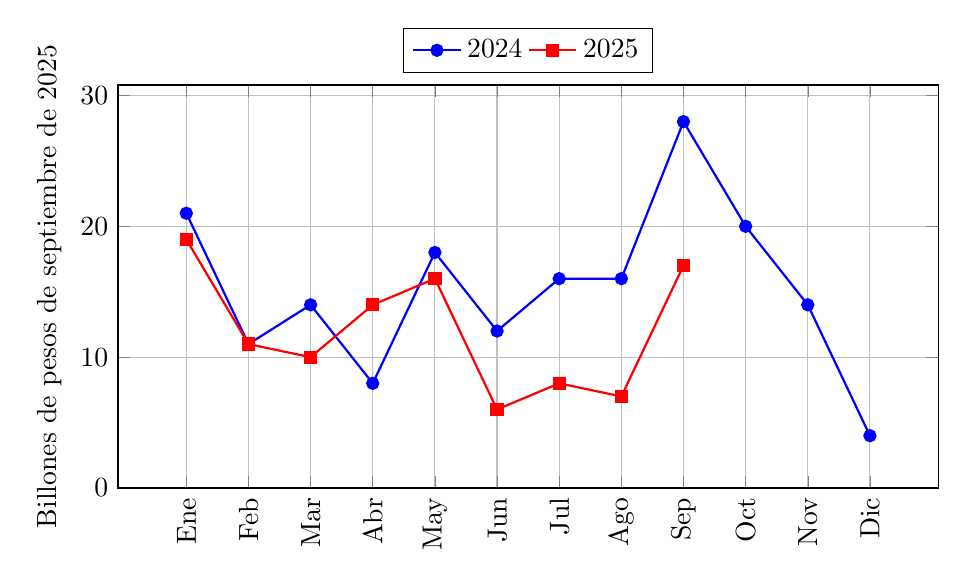
\begin{tikzpicture}
\begin{axis}[
    width=12cm,
    height=6.7cm,
    ylabel={Billones de pesos de septiembre de 2025},
    xtick={1,2,3,4,5,6,7,8,9,10,11,12},
    xticklabels={Ene,Feb,Mar,Abr,May,Jun,Jul,Ago,Sep,Oct,Nov,Dic},
    xticklabel style={rotate=90,anchor=east},
    legend style={at={(0.5,1.03)},anchor=south,legend columns=2},
    grid=both,
    ymin=0
]
\addplot[mark=*,thick,blue] coordinates {(1,21) (2,11) (3,14) (4,8) (5,18) (6,12) (7,16) (8,16) (9,28) (10,20) (11,14) (12,4)};
\addlegendentry{2024}
\addplot[mark=square*,thick,red] coordinates {(1,19) (2,11) (3,10) (4,14) (5,16) (6,6) (7,8) (8,7) (9,17)};
\addlegendentry{2025}
\end{axis}
\end{tikzpicture}
\scriptsize Corte de 2025: septiembre.
\note{[Sources] Dirección General de Crédito Público y Tesoro Nacional, serie conservada de la lámina de liquidez de la versión fuente. El MFMP 2026 no publica esta serie mensual.}
\end{frame}